\chapter{Organisation}
Dette afsnit vil give et indblik i strukturen og opbygningen af Kvindeafdelingen, Svangre- og ultralydsambulatorium på Hospitalsenheden Horsens og afdeling Kvindesygdomme og fødsler på Regionshospitalet Viborg. Afsnittet vil belyse, hvilken betydning implementeringen af en ultralyds robotarm, vil have for afdelingerne som organisation, samt hvilke ændringer dette vil medføre i arbejdsgangen for personalet. \\
Informationer, som er indhentet fra afdelingen på Hospitalsenheden Horsens og afdelingen på Regionshospitalet Viborg, vil blive sammenholdt med videnskabelige artikler, i forsøget på at finde en større sammenhæng i problemstillingen omkring arbejdsgener ved ultralydsscannings arbejdet.

Det er valgt, at benyttes Leavitts organisationsmodel \ref{LeavittModel}, som analysemetode. Denne model er en diamantmodel, der arbejder med fire organisatoriske hovedelementer, der relaterer sig til hinanden. Hvert hovedelement vil blive belyst i hvert sit underafsnit. \cite{EMU2016}

\begin{figure}[h!]\centering
	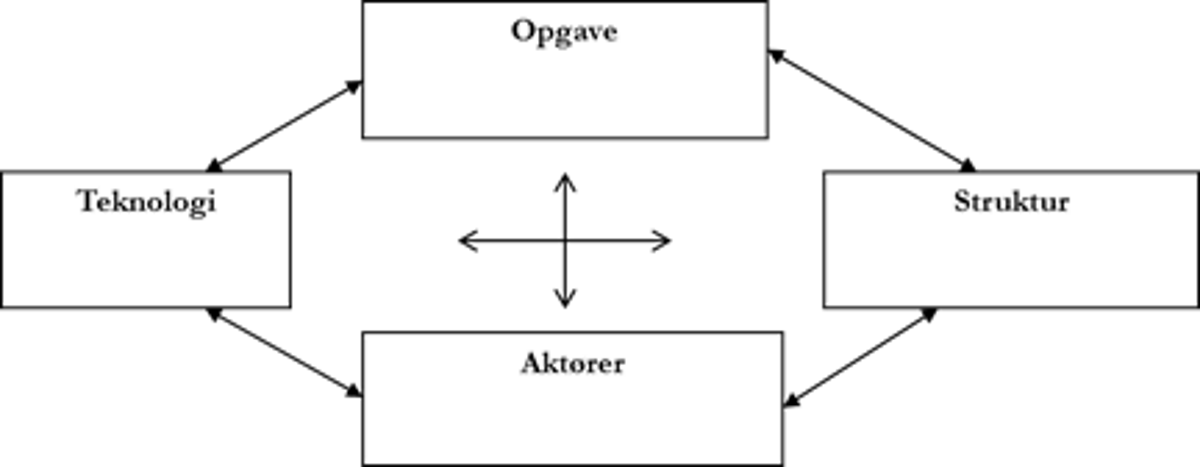
\includegraphics[width = 0.5\textwidth]{Figurer/LeavittModel}
	\caption{Leavitts organisations model, viser hvordan struktur, aktører, opgaver og teknologi indbyrdes relaterer sig til hinanden, i midten haves kulturen for organisationen.}
	\label{LeavittModel}
\end{figure}
I analysen er der kun medtaget to ultralydsafdeling, og derfor er der ikke videre empiri for at kunne drage konklusioner om at billedet vil være det samme på andre lignende hospitals afdelinger i Danmark. 

Dataindsamlingen til analyse er indhentet gennem interview med afdelingssygeplejerske Tina Arnbjørn og tre sonografer fra Hospitalsenheden Horsens, samt interview med afdelingssygeplejerske Karen Marie Goul og en sonograf fra Regionshospitalet Viborg.
Til at underbygge arbejdsskadeproblemstillingen benyttes yderligere videnskabelige artikler.

\section{Kvindeafdelingen, Svangre- og ultralydsambulatorium, Hospitalsenheden Horsens}
Afdelingen på Horsens er bemandet af en afdelingssygeplejerske, fem sonografer samt et ukendt antal læger. Afdelingen har udstyr til fire stuer, hvoraf tre stuer bemandes af sonografer. Der foretages 30-40 scanninger om dagen på afdelingen, hver scanning tager i gennemsnit 35 minutter.

\section{Kvindesygdomme og fødsler, Regionshospitalet Viborg}
Bemanding på afdelingen i Viborg består af en afdelingssygeplejerske, ni sonografer og et ukendt antal læger. Afdelingen har ultralyds scannings udstyr til fem stuer til gravide, hvoraf tre stuer er i drift dagligt og bemandes af sonografer. Dagligt foretages der 25-30 scanninger på afdelingen. En scanning tager i gennemsnittet 30 minutter.

Antallet af læger er ikke relevant for denne analyse, da der udelukkende fokuseres på sonografernes arbejdsgange.

\section{Leavitts organisationsmodel}
Skriv at data sammenskrives, så der ikke gentages. 

\subsection{Opgaver}
Opgaverne som afdelingerne varetager på nuværende tidspunkt, vil ikke ændrer sig ved implementering af robotarmen, da behovet for scanninger af gravide forbliver uændret. Opgaverne består af nakkefoldsscanning i 11.-13. uge, misdannelsesscanning i 19.-22. uge, vægtscanninger samt andre kontrolscanninger i løbet af graviditeten. \cite{Bergholt2014}

\subsection{Teknologi}
Ved implementering af ny teknologi, som ultralyds robotarmen, vil det sætte krav til aktørernes faglige kundskaber og erfaringer i brugen af teknologien. Dette er gældende for samtlige sonografer. Derfor vil der skulle være en indkørselsperiode af teknologien førend, at den vil være i fuld brug og alt personale har den rette kendskab i brugen af robotarmenen. \\
Det vurderes, at de eksisterende stuer på afdelingen i Horsens og i Viborg er tilstrækkelig store til at teknologien vil kunne implementeres uden yderligere ændringer. I Viborg kan det dog blive nødvendigt at flytte patientskærmen, da robotarmstativet muligvis vil komme til at dække for udsynet til skærmen.  

\subsection{Struktur}
På nuværende tidspunkt er den strukturelle opbygning på afdelingen i Horsens, at en medarbejder ultralydsscanner 30 timer ud af 37 timer på en uge. De resterende timer udmønter sig som en aflastnings dag for den enkelte medarbejder, da det er et kendt problem på afdelingen i Horsens at scanningsarbejde er fysisk belastende for medarbejderen. I løbet af en scanningsdag har en medarbejder i gennemsnit ti scanninger. Yderligere foretages der på afdelingen forebyggende tiltag, i form af styrketrænende elastikøvelser, ergonomiske redskaber samt fri adgang til wellness konsulenter, der kontrollerer og vejleder om medarbejderens arbejdsstillinger. (reference)

Implementering af robotarmen vil føre til en ændring i afdelingens strukturelle opbygning for afdelingen i Horsens. Da robotarmen vil kunne gøre scanningsarbejdet væsentlig mindre belastende (reference), vil en medarbejder kunne scanne 5 ud af 5 arbejdsdage om ugen.  

Artikler der underbygger anbefalingerne, og hvornår indtræffer en arbejdsskade typisk. 

\subsection{Aktører}
Implementeringen af robotarmen vil føre til markante ændringer for den enkelte sonografs arbejde.

BMI-problemer (ref. statistik), akavede arbejdsstilling (ref. artikler), fysisk belastende, ikke fuldføre arbejdet over tid (ref. udsagn), dedikerede i jobbet - gemmer arbejdsgener væk (ref. artikler + udsagn).

Definition af arbejdsskade typer, med billeder fra artikler. 

\subsection{Kultur}
Kulturen på afdelingen i Horsens er meget teknologivenlig. Derfor formodes det, at implementeringen af teknologien ikke vil føre til væsentlige problemer i forhold til at få personalet til at benyttes den nye teknologi. Dog kræves det, at der tilrettelægges en ordentlig plan for oplæring af personalet i brugen af teknologien. 

Afdelingen i Horsens har allerede på nuværende tidspunkt indvilliget i at være testafdeling for Robotic Ultrasound ApS under udviklingen af produktet. Det er i afdelingen interesse, da de ser en fremtid i produktet og dermed ønsker at være med til at tilpasse produktet til afdelingens struktur og behov.   

Skriv afsnittet om til at være generelt. 

\section{Delkonklusion}

